\documentclass[a4paper, 11pt]{article}
\usepackage[utf8]{inputenc}
\usepackage{mathtools}
\usepackage{amsmath}
\usepackage{titlesec}
\usepackage{amssymb}
\usepackage{gensymb}
\usepackage[english]{babel}
\usepackage[dvipsnames]{xcolor}
\usepackage[margin=1in]{geometry}
\usepackage[hidelinks]{hyperref}
\usepackage{fancyhdr}
\usepackage{graphicx}
\usepackage{cancel}
\usepackage{float}
\usepackage{subcaption}
\usepackage{tabto}
\usepackage{tocloft}
\usepackage{xcolor}
\usepackage{yfonts}
\usepackage[style=numeric-comp, sorting=none]{biblatex}
\bibliography{bib.bib}
\newcommand{\figuretag}[1]{%
  \addtocounter{figure}{-1}%
  \renewcommand{\thefigure}{#1}%
}

\setcounter{tocdepth}{1}
\renewcommand{\cftdot}{.}

% Configurar las cabeceras para todas las páginas
\pagestyle{fancy}
\lhead{Entrega 1}
\rhead{}

% Para que la cabecera aparezca también en la primera página
\fancypagestyle{plain}{%
  \fancyhf{} % Limpiar cabeceras y pies de página
  \lhead{Entrega 1} % Añadir la cabecera en la primera página
  \rhead{} % Vaciar la cabecera derecha
}

\title{{\textbf{\Large ENTREGA 1: DIFRACCIÓ
}\\}}

\author{Reina Delgado, Airan (1670808)\\}

\date{}

\begin{document}

\maketitle

%%%%%%%%%%%%%%%%%%%%%%%%%%%%%%%%%%%%%%%%%%%%%%%%%%%%%%%%
%%%%%%%%%%%%%%%%%%%%%%%%%%%%%%%%%%%%%%%%%%%%%%%%%%%%%%%%
%%%%%%%%%%%%%%%%%%%%%%%%%%%%%%%%%%%%%%%%%%%%%%%%%%%%%%%%
%%%%%%%%%%%%%%%%%%%%%%%%%%%%%%%%%%%%%%%%%%%%%%%%%%%%%%%%
%%%%%%%%%%%%%%%%%%%%%%%%%%%%%%%%%%%%%%%%%%%%%%%%%%%%%%%%

\noindent Aquesta entrega tracta sobre l'anàlisi de dades obtingudes a partir d'un patró de difracció de raigs X ($\lambda = 1.5406 \text{\AA}$) d'un material cristal·lí d'estructura desconeguda. Els objectius són determinar quina estructura ajusta millor les dades experimentals i trobar la constant de xarxa $a$ del material. En la figura \ref{fig:patro} es mostra el patró de difracció obtingut.

\begin{figure}[h!]
    \centering
    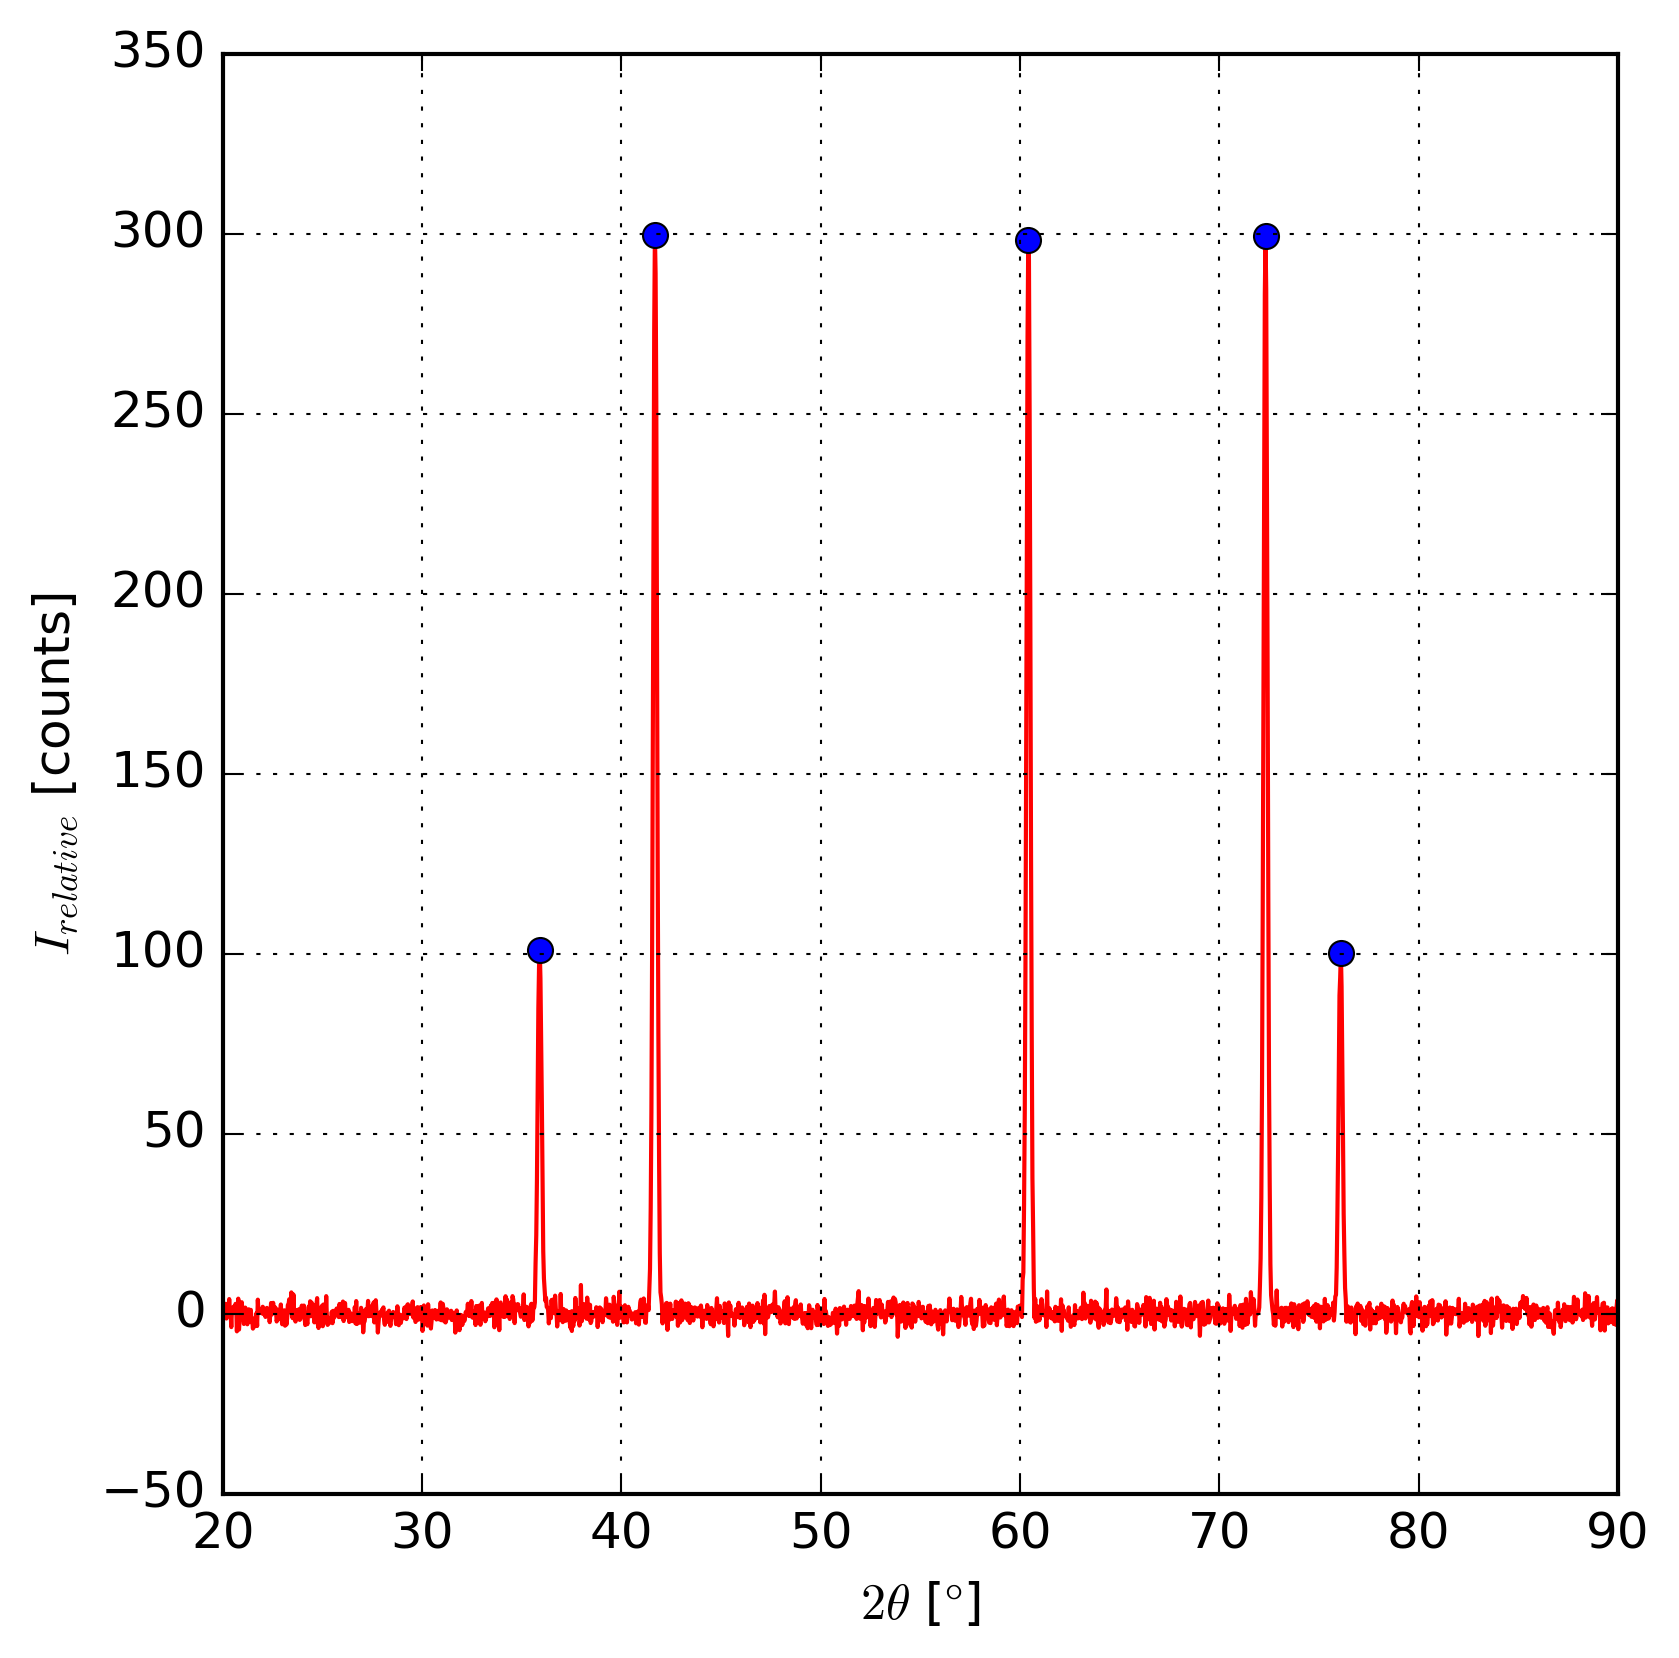
\includegraphics[width=0.7\textwidth]{images/grafic_experimental_peaks.png}
    \caption{Patró de difracció de raigs X obtingut experimentalment.}
    \label{fig:patro}
\end{figure}

\noindent Per realitzar l'anàlisi, s'ha emprat la funció "\textit{find\_peaks}" de la llibreria "\textit{scipy.signal}" per identificar els pics en el patró de difracció. Aquesta funció permet detectar els màxims locals en una sèrie de dades, facilitant la identificació dels angles de difracció corresponents als diferents plans cristal·lins. Per comprovar la veracitat dels pics de forma qualitativa, s'han representat sobre el patró de difracció, com es pot observar. Emprant aquets valors, podem convertir els angles de difracció $\theta$ en les separacions entre plans $d$ mitjançant la llei de Bragg:

\begin{equation}
    2d\sin(\theta) = n\lambda
\end{equation}

\noindent Ón $n$ és l'ordre de difracció (en aquest cas, $n=1$). Els valors tractats en aquesta discussió es poden trobar a la taula \ref{tab:valors}.
\vspace{15mm}

\begin{table}[h!]
    \centering
    \begin{tabular}{|c|c|c|}
        \hline
        Pic & $\theta$ (º) & $d$ (\AA) \\
        \hline
        1 & 17.95 & 2.50 \\
        2 & 20.84 & 2.17 \\
        3 & 30.21 & 1.53 \\
        4 & 36.16 & 1.31 \\
        5 & 38.05 & 1.25 \\
        \hline
    \end{tabular}
    \caption{Magnituds rellevants extretes experimentalment.}
    \label{tab:valors}
\end{table}

\noindent A continuació, es calcula el factor $1/d^2$ per a cada pic, ja que aquest és el que ajusta les diferents estructures cristal·lines considerades. Això es deu a que la relació entre $1/d^2$ i el modul del vector recíproc generic $\vec{G}$ ($|\vec{G}| = h^2 + k^2 + l^2$) d'una xarxa cúbica és lineal, on $h$, $k$ i $l$ són els índexs dels plans cristal·lins de difracció. Si l'estructura és cúbica simple (SC), s'observarien pics en tots els valors de $h$, $k$ i $l$ (Obviant, obviament, les combinacions $(h,k,l)$ que generen vectors proporcionals), mentre que per a les altres estructures (Considerarem cúbica centrada en el cos (BCC), cúbica centrada en les cares (FCC) i diamant) només es permeten certes combinacions d'índexs ja que l'adició d'àtoms en posicions específiques dins de la cel·la unitària provoca interferències destructives que cancel·len alguns pics de difracció. La relació esmentada és la següent:

\begin{equation}
    \frac{1}{d^2} = \frac{h^2 + k^2 + l^2}{a^2}
\end{equation}

\noindent És important observar que la constant de proporcionalitat depén de la constant de xarxa $a$ tal que $a = 1/\sqrt{\text{pendent}}$. A continuació s'adjunta una demostració d'aquesta relació:

%%%%%%%%%%%%%%%%%%%%%%%%%%%%%%%%%%%%%%%%%%%%%%%%%%%%%%%%
%%%%%%%%%%%%%%%%%%%%%%%%%%%%%%%%%%%%%%%%%%%%%%%%%%%%%%%%
%%%%%%%%%%%%%%%%%%%%%%%%%%%%%%%%%%%%%%%%%%%%%%%%%%%%%%%%
%%%%%%%%%%%%%%%%%%%%%%%%%%%%%%%%%%%%%%%%%%%%%%%%%%%%%%%%
%%%%%%%%%%%%%%%%%%%%%%%%%%%%%%%%%%%%%%%%%%%%%%%%%%%%%%%%

\end{document}